\chapter{Những điều cơ bản về đồ thị}

Nhiều bài toán lập trình có thể được giải quyết bằng cách
mô hình hóa bài toán thành một bài toán đồ thị
và sử dụng một thuật toán đồ thị thích hợp.
Một ví dụ điển hình của đồ thị là một mạng lưới
đường và thành phố trong một quốc gia.
Tuy nhiên, đôi khi, đồ thị bị ẩn
trong bài toán và có thể khó phát hiện ra nó.

Phần này của cuốn sách thảo luận về các thuật toán đồ thị,
đặc biệt tập trung vào các chủ đề
quan trọng trong lập trình thi đấu.
Trong chương này, chúng ta sẽ tìm hiểu các khái niệm
liên quan đến đồ thị,
và nghiên cứu các cách khác nhau để biểu diễn đồ thị trong các thuật toán.

\section{Thuật ngữ đồ thị}

\index{đồ thị}
\index{nút}
\index{cạnh}

Một \key{đồ thị} bao gồm các \key{nút}
và \key{cạnh}. Trong cuốn sách này,
biến $n$ biểu thị số lượng nút
trong một đồ thị, và biến $m$ biểu thị
số lượng cạnh.
Các nút được đánh số
bằng các số nguyên $1,2,\ldots,n$.

Ví dụ, đồ thị sau bao gồm 5 nút và 7 cạnh:

\begin{center}
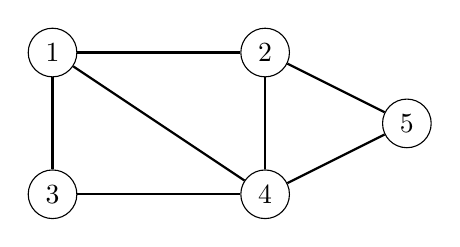
\begin{tikzpicture}[scale=0.9]
\node[draw, circle] (1) at (1,3) {$1$};
\node[draw, circle] (2) at (4,3) {$2$};
\node[draw, circle] (3) at (1,1) {$3$};
\node[draw, circle] (4) at (4,1) {$4$};
\node[draw, circle] (5) at (6,2) {$5$};

\path[draw,thick,-] (1) -- (2);
\path[draw,thick,-] (1) -- (3);
\path[draw,thick,-] (1) -- (4);
\path[draw,thick,-] (3) -- (4);
\path[draw,thick,-] (2) -- (4);
\path[draw,thick,-] (2) -- (5);
\path[draw,thick,-] (4) -- (5);
\end{tikzpicture}
\end{center}

\index{đường đi}

Một \key{đường đi} dẫn từ nút $a$ đến nút $b$
qua các cạnh của đồ thị.
\key{Độ dài} của một đường đi là số lượng
cạnh trong đó.
Ví dụ, đồ thị trên chứa
một đường đi $1 \rightarrow 3 \rightarrow 4 \rightarrow 5$
có độ dài 3
từ nút 1 đến nút 5:

\begin{center}
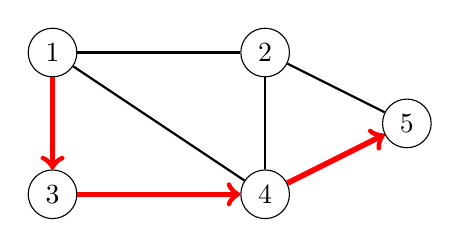
\begin{tikzpicture}[scale=0.9]
\node[draw, circle] (1) at (1,3) {$1$};
\node[draw, circle] (2) at (4,3) {$2$};
\node[draw, circle] (3) at (1,1) {$3$};
\node[draw, circle] (4) at (4,1) {$4$};
\node[draw, circle] (5) at (6,2) {$5$};

\path[draw,thick,-] (1) -- (2);
\path[draw,thick,-] (1) -- (3);
\path[draw,thick,-] (1) -- (4);
\path[draw,thick,-] (3) -- (4);
\path[draw,thick,-] (2) -- (4);
\path[draw,thick,-] (2) -- (5);
\path[draw,thick,-] (4) -- (5);

\path[draw=red,thick,->,line width=2pt] (1) -- (3);
\path[draw=red,thick,->,line width=2pt] (3) -- (4);
\path[draw=red,thick,->,line width=2pt] (4) -- (5);
\end{tikzpicture}
\end{center}

\index{chu trình}

Một đường đi là một \key{chu trình} nếu nút đầu tiên và cuối cùng
giống nhau.
Ví dụ, đồ thị trên chứa
một chu trình $1 \rightarrow 3 \rightarrow 4 \rightarrow 1$.
Một đường đi là \key{đơn giản} nếu mỗi nút xuất hiện
nhiều nhất một lần trong đường đi.


% 
% \begin{itemize}
% \item $1 \rightarrow 2 \rightarrow 5$ (length 2)
% \item $1 \rightarrow 4 \rightarrow 5$ (length 2)
% \item $1 \rightarrow 2 \rightarrow 4 \rightarrow 5$ (length 3)
% \item $1 \rightarrow 3 \rightarrow 4 \rightarrow 5$ (length 3)
% \item $1 \rightarrow 4 \rightarrow 2 \rightarrow 5$ (length 3)
% \item $1 \rightarrow 3 \rightarrow 4 \rightarrow 2 \rightarrow 5$ (length 4)
% \end{itemize}

\subsubsection{Tính liên thông}

\index{đồ thị liên thông}

Một đồ thị là \key{liên thông} nếu có một đường đi
giữa bất kỳ hai nút nào.
Ví dụ, đồ thị sau là liên thông:
\begin{center}
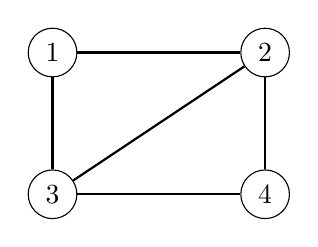
\begin{tikzpicture}[scale=0.9]
\node[draw, circle] (1) at (1,3) {$1$};
\node[draw, circle] (2) at (4,3) {$2$};
\node[draw, circle] (3) at (1,1) {$3$};
\node[draw, circle] (4) at (4,1) {$4$};
\path[draw,thick,-] (1) -- (2);
\path[draw,thick,-] (1) -- (3);
\path[draw,thick,-] (2) -- (3);
\path[draw,thick,-] (3) -- (4);
\path[draw,thick,-] (2) -- (4);
\end{tikzpicture}
\end{center}

Đồ thị sau không liên thông,
vì không thể đi
từ nút 4 đến bất kỳ nút nào khác:
\begin{center}
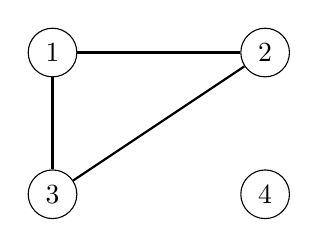
\begin{tikzpicture}[scale=0.9]
\node[draw, circle] (1) at (1,3) {$1$};
\node[draw, circle] (2) at (4,3) {$2$};
\node[draw, circle] (3) at (1,1) {$3$};
\node[draw, circle] (4) at (4,1) {$4$};
\path[draw,thick,-] (1) -- (2);
\path[draw,thick,-] (1) -- (3);
\path[draw,thick,-] (2) -- (3);
\end{tikzpicture}
\end{center}

\index{thành phần}

Các phần liên thông của một đồ thị được
gọi là các \key{thành phần} của nó.
Ví dụ, đồ thị sau
chứa ba thành phần:
$\{1,\,2,\,3\}$,
$\{4,\,5,\,6,\,7\}$ và
$\{8\}$.
\begin{center}
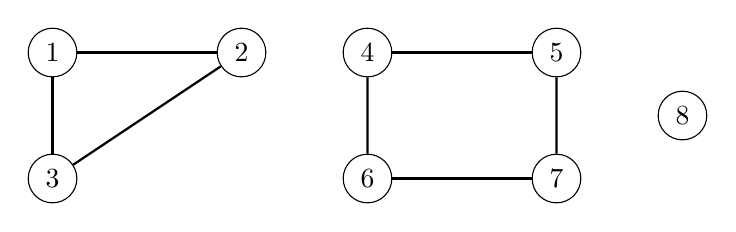
\begin{tikzpicture}[scale=0.8]
\node[draw, circle] (1) at (1,3) {$1$};
\node[draw, circle] (2) at (4,3) {$2$};
\node[draw, circle] (3) at (1,1) {$3$};

\node[draw, circle] (6) at (6,1) {$6$};
\node[draw, circle] (7) at (9,1) {$7$};
\node[draw, circle] (4) at (6,3) {$4$};
\node[draw, circle] (5) at (9,3) {$5$};

\node[draw, circle] (8) at (11,2) {$8$};

\path[draw,thick,-] (1) -- (2);
\path[draw,thick,-] (2) -- (3);
\path[draw,thick,-] (1) -- (3);
\path[draw,thick,-] (4) -- (5);
\path[draw,thick,-] (5) -- (7);
\path[draw,thick,-] (6) -- (7);
\path[draw,thick,-] (6) -- (4);
\end{tikzpicture}
\end{center}

\index{cây}

Một \key{cây} là một đồ thị liên thông
bao gồm $n$ nút và $n-1$ cạnh.
Có một đường đi duy nhất
giữa bất kỳ hai nút nào của một cây.
Ví dụ, đồ thị sau là một cây:

\begin{center}
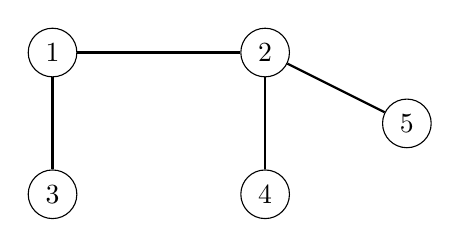
\begin{tikzpicture}[scale=0.9]
\node[draw, circle] (1) at (1,3) {$1$};
\node[draw, circle] (2) at (4,3) {$2$};
\node[draw, circle] (3) at (1,1) {$3$};
\node[draw, circle] (4) at (4,1) {$4$};
\node[draw, circle] (5) at (6,2) {$5$};

\path[draw,thick,-] (1) -- (2);
\path[draw,thick,-] (1) -- (3);
%\path[draw,thick,-] (1) -- (4);
\path[draw,thick,-] (2) -- (5);
\path[draw,thick,-] (2) -- (4);
%\path[draw,thick,-] (4) -- (5);
\end{tikzpicture}
\end{center}

\subsubsection{Hướng cạnh}

\index{đồ thị có hướng}

Một đồ thị là \key{có hướng}
nếu các cạnh chỉ có thể được đi qua
theo một hướng duy nhất.
Ví dụ, đồ thị sau là có hướng:
\begin{center}
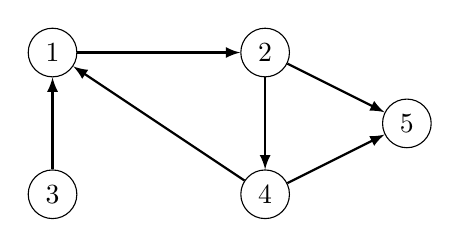
\begin{tikzpicture}[scale=0.9]
\node[draw, circle] (1) at (1,3) {$1$};
\node[draw, circle] (2) at (4,3) {$2$};
\node[draw, circle] (3) at (1,1) {$3$};
\node[draw, circle] (4) at (4,1) {$4$};
\node[draw, circle] (5) at (6,2) {$5$};
\path[draw,thick,->,>=latex] (1) -- (2);
\path[draw,thick,->,>=latex] (2) -- (4);
\path[draw,thick,->,>=latex] (2) -- (5);
\path[draw,thick,->,>=latex] (4) -- (5);
\path[draw,thick,->,>=latex] (4) -- (1);
\path[draw,thick,->,>=latex] (3) -- (1);
\end{tikzpicture}
\end{center}

Đồ thị trên chứa
một đường đi $3 \rightarrow 1 \rightarrow 2 \rightarrow 5$
từ nút $3$ đến nút $5$,
nhưng không có đường đi từ nút $5$ đến nút $3$.

\subsubsection{Trọng số cạnh}

\index{đồ thị có trọng số}

Trong một đồ thị \key{có trọng số}, mỗi cạnh được gán
một \key{trọng số}.
Các trọng số thường được hiểu là độ dài cạnh.
Ví dụ, đồ thị sau là có trọng số:
\begin{center}
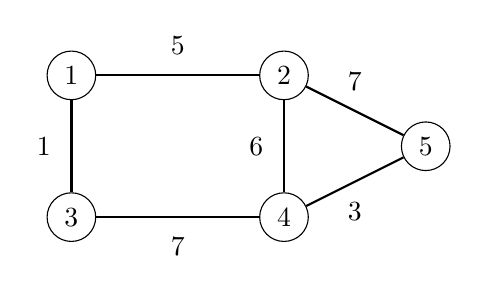
\begin{tikzpicture}[scale=0.9]
\node[draw, circle] (1) at (1,3) {$1$};
\node[draw, circle] (2) at (4,3) {$2$};
\node[draw, circle] (3) at (1,1) {$3$};
\node[draw, circle] (4) at (4,1) {$4$};
\node[draw, circle] (5) at (6,2) {$5$};
\path[draw,thick,-] (1) -- node[font=\small,label=above:5] {} (2);
\path[draw,thick,-] (1) -- node[font=\small,label=left:1] {} (3);
\path[draw,thick,-] (3) -- node[font=\small,label=below:7] {} (4);
\path[draw,thick,-] (2) -- node[font=\small,label=left:6] {} (4);
\path[draw,thick,-] (2) -- node[font=\small,label=above:7] {} (5);
\path[draw,thick,-] (4) -- node[font=\small,label=below:3] {} (5);
\end{tikzpicture}
\end{center}

Độ dài của một đường đi trong một đồ thị có trọng số
là tổng của các trọng số cạnh trên đường đi.
Ví dụ, trong đồ thị trên,
độ dài của đường đi
$1 \rightarrow 2 \rightarrow 5$ là $12$,
và độ dài của đường đi
$1 \rightarrow 3 \rightarrow 4 \rightarrow 5$ là $11$.
Đường đi sau là đường đi \key{ngắn nhất} từ nút $1$ đến nút $5$.

\subsubsection{Hàng xóm và bậc}

\index{hàng xóm}
\index{bậc}

Hai nút là \key{hàng xóm} hoặc \key{liền kề}
nếu có một cạnh giữa chúng.
\key{Bậc} của một nút
là số lượng hàng xóm của nó.
Ví dụ, trong đồ thị sau,
các hàng xóm của nút 2 là 1, 4 và 5,
vì vậy bậc của nó là 3.

\begin{center}
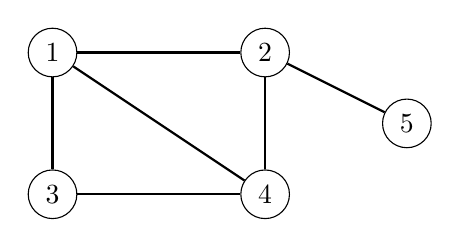
\begin{tikzpicture}[scale=0.9]
\node[draw, circle] (1) at (1,3) {$1$};
\node[draw, circle] (2) at (4,3) {$2$};
\node[draw, circle] (3) at (1,1) {$3$};
\node[draw, circle] (4) at (4,1) {$4$};
\node[draw, circle] (5) at (6,2) {$5$};

\path[draw,thick,-] (1) -- (2);
\path[draw,thick,-] (1) -- (3);
\path[draw,thick,-] (1) -- (4);
\path[draw,thick,-] (3) -- (4);
\path[draw,thick,-] (2) -- (4);
\path[draw,thick,-] (2) -- (5);
%\path[draw,thick,-] (4) -- (5);
\end{tikzpicture}
\end{center}

Tổng các bậc trong một đồ thị luôn là $2m$,
trong đó $m$ là số cạnh,
vì mỗi cạnh
làm tăng bậc của đúng hai nút lên một.
Vì lý do này, tổng các bậc luôn là số chẵn.

\index{đồ thị chính quy}
\index{đồ thị đầy đủ}

Một đồ thị là \key{chính quy} nếu
bậc của mọi nút là một hằng số $d$.
Một đồ thị là \key{đầy đủ} nếu
bậc của mọi nút là $n-1$, tức là,
đồ thị chứa tất cả các cạnh có thể có
giữa các nút.

\index{bán bậc vào}
\index{bán bậc ra}

Trong một đồ thị có hướng, \key{bán bậc vào}
của một nút là số cạnh
kết thúc tại nút đó,
và \key{bán bậc ra} của một nút
là số cạnh bắt đầu từ nút đó.
Ví dụ, trong đồ thị sau,
bán bậc vào của nút 2 là 2,
và bán bậc ra của nút 2 là 1.

\begin{center}
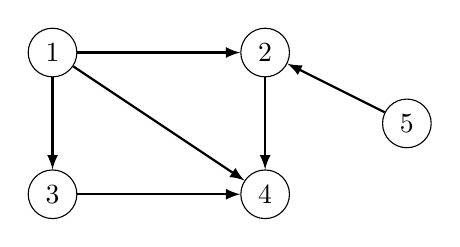
\begin{tikzpicture}[scale=0.9]
\node[draw, circle] (1) at (1,3) {$1$};
\node[draw, circle] (2) at (4,3) {$2$};
\node[draw, circle] (3) at (1,1) {$3$};
\node[draw, circle] (4) at (4,1) {$4$};
\node[draw, circle] (5) at (6,2) {$5$};

\path[draw,thick,->,>=latex] (1) -- (2);
\path[draw,thick,->,>=latex] (1) -- (3);
\path[draw,thick,->,>=latex] (1) -- (4);
\path[draw,thick,->,>=latex] (3) -- (4);
\path[draw,thick,->,>=latex] (2) -- (4);
\path[draw,thick,<-,>=latex] (2) -- (5);
\end{tikzpicture}
\end{center}

\subsubsection{Tô màu}

\index{tô màu}
\index{đồ thị hai phía}

Trong một \key{tô màu} của một đồ thị,
mỗi nút được gán một màu sao cho
không có hai nút liền kề nào có cùng màu.

Một đồ thị là \key{hai phía} nếu
có thể tô màu nó bằng hai màu.
Hóa ra một đồ thị là hai phía
chính xác khi nó không chứa một chu trình
với số cạnh lẻ.
Ví dụ, đồ thị
\begin{center}
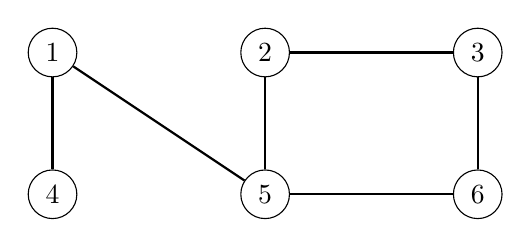
\begin{tikzpicture}[scale=0.9]
\node[draw, circle] (1) at (1,3) {$2$};
\node[draw, circle] (2) at (4,3) {$3$};
\node[draw, circle] (3) at (1,1) {$5$};
\node[draw, circle] (4) at (4,1) {$6$};
\node[draw, circle] (5) at (-2,1) {$4$};
\node[draw, circle] (6) at (-2,3) {$1$};
\path[draw,thick,-] (1) -- (2);
\path[draw,thick,-] (1) -- (3);
\path[draw,thick,-] (3) -- (4);
\path[draw,thick,-] (2) -- (4);
\path[draw,thick,-] (3) -- (6);
\path[draw,thick,-] (5) -- (6);
\end{tikzpicture}
\end{center}
là hai phía, vì nó có thể được tô màu như sau:
\begin{center}
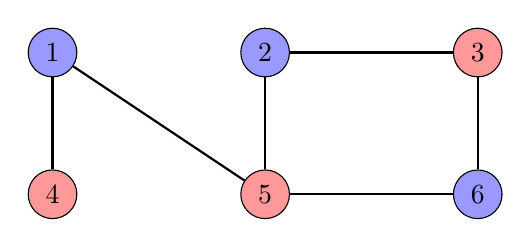
\begin{tikzpicture}[scale=0.9]
\node[draw, circle, fill=blue!40] (1) at (1,3) {$2$};
\node[draw, circle, fill=red!40] (2) at (4,3) {$3$};
\node[draw, circle, fill=red!40] (3) at (1,1) {$5$};
\node[draw, circle, fill=blue!40] (4) at (4,1) {$6$};
\node[draw, circle, fill=red!40] (5) at (-2,1) {$4$};
\node[draw, circle, fill=blue!40] (6) at (-2,3) {$1$};
\path[draw,thick,-] (1) -- (2);
\path[draw,thick,-] (1) -- (3);
\path[draw,thick,-] (3) -- (4);
\path[draw,thick,-] (2) -- (4);
\path[draw,thick,-] (3) -- (6);
\path[draw,thick,-] (5) -- (6);
\end{tikzpicture}
\end{center}
Tuy nhiên, đồ thị
\begin{center}
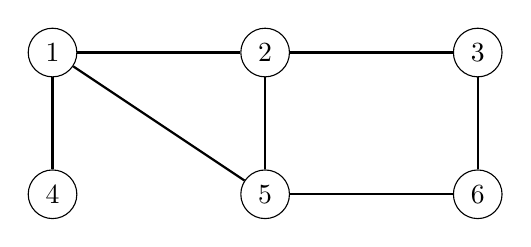
\begin{tikzpicture}[scale=0.9]
\node[draw, circle] (1) at (1,3) {$2$};
\node[draw, circle] (2) at (4,3) {$3$};
\node[draw, circle] (3) at (1,1) {$5$};
\node[draw, circle] (4) at (4,1) {$6$};
\node[draw, circle] (5) at (-2,1) {$4$};
\node[draw, circle] (6) at (-2,3) {$1$};
\path[draw,thick,-] (1) -- (2);
\path[draw,thick,-] (1) -- (3);
\path[draw,thick,-] (3) -- (4);
\path[draw,thick,-] (2) -- (4);
\path[draw,thick,-] (3) -- (6);
\path[draw,thick,-] (5) -- (6);
\path[draw,thick,-] (1) -- (6);
\end{tikzpicture}
\end{center}
không phải là hai phía, vì không thể tô màu
chu trình sau gồm ba nút bằng hai màu:
\begin{center}
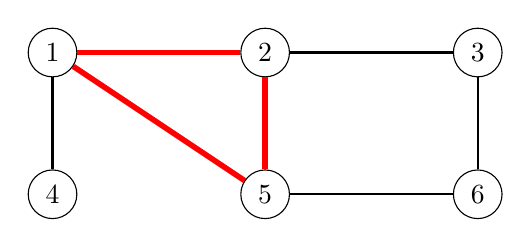
\begin{tikzpicture}[scale=0.9]
\node[draw, circle] (1) at (1,3) {$2$};
\node[draw, circle] (2) at (4,3) {$3$};
\node[draw, circle] (3) at (1,1) {$5$};
\node[draw, circle] (4) at (4,1) {$6$};
\node[draw, circle] (5) at (-2,1) {$4$};
\node[draw, circle] (6) at (-2,3) {$1$};
\path[draw,thick,-] (1) -- (2);
\path[draw,thick,-] (1) -- (3);
\path[draw,thick,-] (3) -- (4);
\path[draw,thick,-] (2) -- (4);
\path[draw,thick,-] (3) -- (6);
\path[draw,thick,-] (5) -- (6);
\path[draw,thick,-] (1) -- (6);

\path[draw=red,thick,-,line width=2pt] (1) -- (3);
\path[draw=red,thick,-,line width=2pt] (3) -- (6);
\path[draw=red,thick,-,line width=2pt] (6) -- (1);
\end{tikzpicture}
\end{center}

\subsubsection{Tính đơn giản}

\index{đồ thị đơn}

Một đồ thị là \key{đơn}
nếu không có cạnh nào bắt đầu và kết thúc tại cùng một nút,
và không có nhiều
cạnh giữa hai nút.
Thường thì chúng ta giả định rằng các đồ thị là đơn.
Ví dụ, đồ thị sau \emph{không} đơn:
\begin{center}
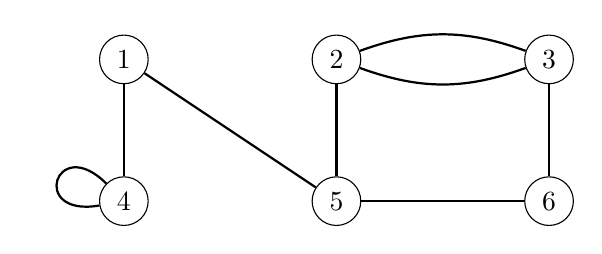
\begin{tikzpicture}[scale=0.9]
\node[draw, circle] (1) at (1,3) {$2$};
\node[draw, circle] (2) at (4,3) {$3$};
\node[draw, circle] (3) at (1,1) {$5$};
\node[draw, circle] (4) at (4,1) {$6$};
\node[draw, circle] (5) at (-2,1) {$4$};
\node[draw, circle] (6) at (-2,3) {$1$};

\path[draw,thick,-] (1) edge [bend right=20] (2);
\path[draw,thick,-] (2) edge [bend right=20] (1);
%\path[draw,thick,-] (1) -- (2);
\path[draw,thick,-] (1) -- (3);
\path[draw,thick,-] (3) -- (4);
\path[draw,thick,-] (2) -- (4);
\path[draw,thick,-] (3) -- (6);
\path[draw,thick,-] (5) -- (6);

\tikzset{every loop/.style={in=135,out=190}}
\path[draw,thick,-] (5) edge [loop left] (5);
\end{tikzpicture}
\end{center}

\section{Biểu diễn đồ thị}

Có một số cách để biểu diễn đồ thị
trong các thuật toán.
Việc lựa chọn một cấu trúc dữ liệu
phụ thuộc vào kích thước của đồ thị và
cách thuật toán xử lý nó.
Tiếp theo, chúng ta sẽ xem xét ba cách biểu diễn phổ biến.

\subsubsection{Biểu diễn danh sách kề}

\index{danh sách kề}

Trong biểu diễn danh sách kề,
mỗi nút $x$ trong đồ thị được gán một \key{danh sách kề}
bao gồm các nút
mà có một cạnh từ $x$ đến chúng.
Danh sách kề là cách phổ biến nhất
để biểu diễn đồ thị, và hầu hết các thuật toán có thể được
thực hiện hiệu quả bằng cách sử dụng chúng.

Một cách thuận tiện để lưu trữ các danh sách kề là khai báo
một mảng các vector như sau:
\begin{lstlisting}
vector<int> adj[N];
\end{lstlisting}

Hằng số $N$ được chọn sao cho tất cả
các danh sách kề có thể được lưu trữ.
Ví dụ, đồ thị

\begin{center}
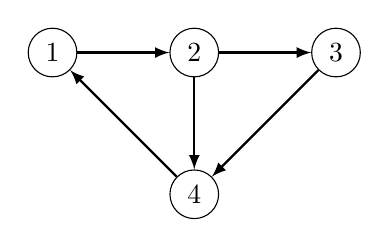
\begin{tikzpicture}[scale=0.9]
\node[draw, circle] (1) at (1,3) {$1$};
\node[draw, circle] (2) at (3,3) {$2$};
\node[draw, circle] (3) at (5,3) {$3$};
\node[draw, circle] (4) at (3,1) {$4$};

\path[draw,thick,->,>=latex] (1) -- (2);
\path[draw,thick,->,>=latex] (2) -- (3);
\path[draw,thick,->,>=latex] (2) -- (4);
\path[draw,thick,->,>=latex] (3) -- (4);
\path[draw,thick,->,>=latex] (4) -- (1);
\end{tikzpicture}
\end{center}
có thể được lưu trữ như sau:
\begin{lstlisting}
adj[1].push_back(2);
adj[2].push_back(3);
adj[2].push_back(4);
adj[3].push_back(4);
adj[4].push_back(1);
\end{lstlisting}

Nếu đồ thị là vô hướng, nó có thể được lưu trữ theo cách tương tự,
nhưng mỗi cạnh được thêm vào theo cả hai hướng.

Đối với một đồ thị có trọng số, cấu trúc có thể được mở rộng
như sau:

\begin{lstlisting}
vector<pair<int,int>> adj[N];
\end{lstlisting}

Trong trường hợp này, danh sách kề của nút $a$
chứa cặp $(b,w)$
luôn luôn khi có một cạnh từ nút $a$ đến nút $b$
với trọng số $w$. Ví dụ, đồ thị

\begin{center}
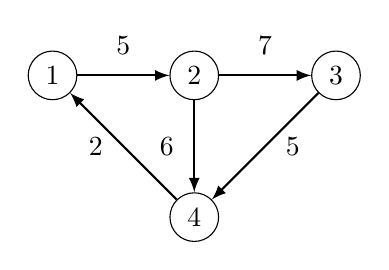
\begin{tikzpicture}[scale=0.9]
\node[draw, circle] (1) at (1,3) {$1$};
\node[draw, circle] (2) at (3,3) {$2$};
\node[draw, circle] (3) at (5,3) {$3$};
\node[draw, circle] (4) at (3,1) {$4$};

\path[draw,thick,->,>=latex] (1) -- node[font=\small,label=above:5] {} (2);
\path[draw,thick,->,>=latex] (2) -- node[font=\small,label=above:7] {} (3);
\path[draw,thick,->,>=latex] (2) -- node[font=\small,label=left:6] {} (4);
\path[draw,thick,->,>=latex] (3) -- node[font=\small,label=right:5] {} (4);
\path[draw,thick,->,>=latex] (4) -- node[font=\small,label=left:2] {} (1);
\end{tikzpicture}
\end{center}
có thể được lưu trữ như sau:
\begin{lstlisting}
adj[1].push_back({2,5});
adj[2].push_back({3,7});
adj[2].push_back({4,6});
adj[3].push_back({4,5});
adj[4].push_back({1,2});
\end{lstlisting}

Lợi ích của việc sử dụng danh sách kề là
chúng ta có thể tìm thấy hiệu quả các nút mà
chúng ta có thể di chuyển đến từ một nút đã cho thông qua một cạnh.
Ví dụ, vòng lặp sau duyệt qua tất cả các nút
mà chúng ta có thể di chuyển đến từ nút $s$:

\begin{lstlisting}
for (auto u : adj[s]) {
    // xu ly nut u
}
\end{lstlisting}

\subsubsection{Biểu diễn ma trận kề}

\index{ma trận kề}

Một \key{ma trận kề} là một mảng hai chiều
chỉ ra các cạnh mà đồ thị chứa.
Chúng ta có thể kiểm tra hiệu quả từ một ma trận kề
nếu có một cạnh giữa hai nút.
Ma trận có thể được lưu trữ dưới dạng một mảng
\begin{lstlisting}
int adj[N][N];
\end{lstlisting}
trong đó mỗi giá trị $\texttt{adj}[a][b]$ chỉ ra
liệu đồ thị có chứa một cạnh từ
nút $a$ đến nút $b$ hay không.
Nếu cạnh được bao gồm trong đồ thị,
thì $\texttt{adj}[a][b]=1$,
và ngược lại $\texttt{adj}[a][b]=0$.
Ví dụ, đồ thị
\begin{center}
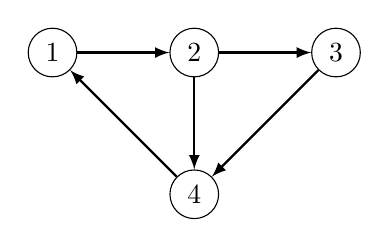
\begin{tikzpicture}[scale=0.9]
\node[draw, circle] (1) at (1,3) {$1$};
\node[draw, circle] (2) at (3,3) {$2$};
\node[draw, circle] (3) at (5,3) {$3$};
\node[draw, circle] (4) at (3,1) {$4$};

\path[draw,thick,->,>=latex] (1) -- (2);
\path[draw,thick,->,>=latex] (2) -- (3);
\path[draw,thick,->,>=latex] (2) -- (4);
\path[draw,thick,->,>=latex] (3) -- (4);
\path[draw,thick,->,>=latex] (4) -- (1);
\end{tikzpicture}
\end{center}
có thể được biểu diễn như sau:
\begin{center}
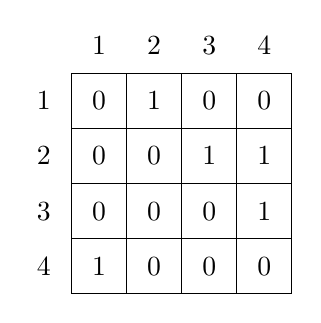
\begin{tikzpicture}[scale=0.7]
\draw (0,0) grid (4,4);
\node at (0.5,0.5) {1};
\node at (1.5,0.5) {0};
\node at (2.5,0.5) {0};
\node at (3.5,0.5) {0};
\node at (0.5,1.5) {0};
\node at (1.5,1.5) {0};
\node at (2.5,1.5) {0};
\node at (3.5,1.5) {1};
\node at (0.5,2.5) {0};
\node at (1.5,2.5) {0};
\node at (2.5,2.5) {1};
\node at (3.5,2.5) {1};
\node at (0.5,3.5) {0};
\node at (1.5,3.5) {1};
\node at (2.5,3.5) {0};
\node at (3.5,3.5) {0};
\node at (-0.5,0.5) {4};
\node at (-0.5,1.5) {3};
\node at (-0.5,2.5) {2};
\node at (-0.5,3.5) {1};
\node at (0.5,4.5) {1};
\node at (1.5,4.5) {2};
\node at (2.5,4.5) {3};
\node at (3.5,4.5) {4};
\end{tikzpicture}
\end{center}

Nếu đồ thị có trọng số, biểu diễn ma trận kề
có thể được mở rộng sao cho
ma trận chứa trọng số của cạnh
nếu cạnh tồn tại.
Sử dụng biểu diễn này, đồ thị

\begin{center}
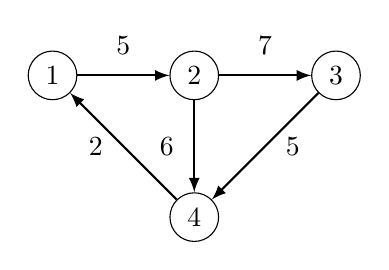
\begin{tikzpicture}[scale=0.9]
\node[draw, circle] (1) at (1,3) {$1$};
\node[draw, circle] (2) at (3,3) {$2$};
\node[draw, circle] (3) at (5,3) {$3$};
\node[draw, circle] (4) at (3,1) {$4$};

\path[draw,thick,->,>=latex] (1) -- node[font=\small,label=above:5] {} (2);
\path[draw,thick,->,>=latex] (2) -- node[font=\small,label=above:7] {} (3);
\path[draw,thick,->,>=latex] (2) -- node[font=\small,label=left:6] {} (4);
\path[draw,thick,->,>=latex] (3) -- node[font=\small,label=right:5] {} (4);
\path[draw,thick,->,>=latex] (4) -- node[font=\small,label=left:2] {} (1);
\end{tikzpicture}
\end{center}
\begin{samepage}
tương ứng với ma trận sau:
\begin{center}
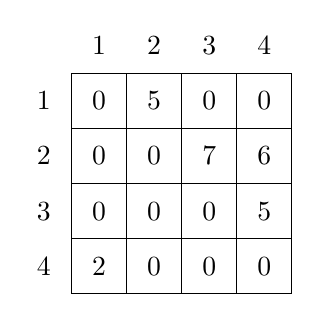
\begin{tikzpicture}[scale=0.7]
\draw (0,0) grid (4,4);
\node at (0.5,0.5) {2};
\node at (1.5,0.5) {0};
\node at (2.5,0.5) {0};
\node at (3.5,0.5) {0};
\node at (0.5,1.5) {0};
\node at (1.5,1.5) {0};
\node at (2.5,1.5) {0};
\node at (3.5,1.5) {5};
\node at (0.5,2.5) {0};
\node at (1.5,2.5) {0};
\node at (2.5,2.5) {7};
\node at (3.5,2.5) {6};
\node at (0.5,3.5) {0};
\node at (1.5,3.5) {5};
\node at (2.5,3.5) {0};
\node at (3.5,3.5) {0};
\node at (-0.5,0.5) {4};
\node at (-0.5,1.5) {3};
\node at (-0.5,2.5) {2};
\node at (-0.5,3.5) {1};
\node at (0.5,4.5) {1};
\node at (1.5,4.5) {2};
\node at (2.5,4.5) {3};
\node at (3.5,4.5) {4};
\end{tikzpicture}
\end{center}
\end{samepage}

Nhược điểm của biểu diễn ma trận kề
là ma trận chứa $n^2$ phần tử,
và thường thì hầu hết chúng là không.
Vì lý do này, biểu diễn này không thể được sử dụng
nếu đồ thị lớn.

\subsubsection{Biểu diễn danh sách cạnh}

\index{danh sách cạnh}

Một \key{danh sách cạnh} chứa tất cả các cạnh của một đồ thị
theo một thứ tự nào đó.
Đây là một cách thuận tiện để biểu diễn một đồ thị
nếu thuật toán xử lý tất cả các cạnh của đồ thị
và không cần tìm các cạnh bắt đầu
tại một nút đã cho.

Danh sách cạnh có thể được lưu trữ trong một vector
\begin{lstlisting}
vector<pair<int,int>> edges;
\end{lstlisting}
trong đó mỗi cặp $(a,b)$ biểu thị rằng
có một cạnh từ nút $a$ đến nút $b$.
Do đó, đồ thị

\begin{center}
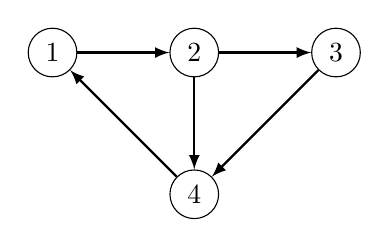
\begin{tikzpicture}[scale=0.9]
\node[draw, circle] (1) at (1,3) {$1$};
\node[draw, circle] (2) at (3,3) {$2$};
\node[draw, circle] (3) at (5,3) {$3$};
\node[draw, circle] (4) at (3,1) {$4$};

\path[draw,thick,->,>=latex] (1) -- (2);
\path[draw,thick,->,>=latex] (2) -- (3);
\path[draw,thick,->,>=latex] (2) -- (4);
\path[draw,thick,->,>=latex] (3) -- (4);
\path[draw,thick,->,>=latex] (4) -- (1);
\end{tikzpicture}
\end{center}
có thể được biểu diễn như sau:
\begin{lstlisting}
edges.push_back({1,2});
edges.push_back({2,3});
edges.push_back({2,4});
edges.push_back({3,4});
edges.push_back({4,1});
\end{lstlisting}

\noindent
Nếu đồ thị có trọng số, cấu trúc có thể
được mở rộng như sau:
\begin{lstlisting}
vector<tuple<int,int,int>> edges;
\end{lstlisting}
Mỗi phần tử trong danh sách này có dạng
$(a,b,w)$, có nghĩa là có
một cạnh từ nút $a$ đến nút $b$ với trọng số $w$.
Ví dụ, đồ thị

\begin{center}
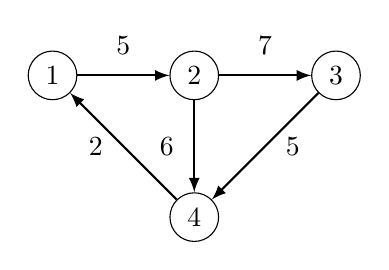
\begin{tikzpicture}[scale=0.9]
\node[draw, circle] (1) at (1,3) {$1$};
\node[draw, circle] (2) at (3,3) {$2$};
\node[draw, circle] (3) at (5,3) {$3$};
\node[draw, circle] (4) at (3,1) {$4$};

\path[draw,thick,->,>=latex] (1) -- node[font=\small,label=above:5] {} (2);
\path[draw,thick,->,>=latex] (2) -- node[font=\small,label=above:7] {} (3);
\path[draw,thick,->,>=latex] (2) -- node[font=\small,label=left:6] {} (4);
\path[draw,thick,->,>=latex] (3) -- node[font=\small,label=right:5] {} (4);
\path[draw,thick,->,>=latex] (4) -- node[font=\small,label=left:2] {} (1);
\end{tikzpicture}
\end{center}
\begin{samepage}
có thể được biểu diễn như sau\footnote{Trong một số trình biên dịch cũ hơn, hàm
\texttt{make\_tuple} phải được sử dụng thay vì dấu ngoặc nhọn (ví dụ,
\texttt{make\_tuple(1,2,5)} thay vì \texttt{\{1,2,5\}}).}:
\begin{lstlisting}
edges.push_back({1,2,5});
edges.push_back({2,3,7});
edges.push_back({2,4,6});
edges.push_back({3,4,5});
edges.push_back({4,1,2});
\end{lstlisting}
\end{samepage}
